\documentclass[a4paper,12pt]{article} 

%%% Работа с русским языком
\usepackage{cmap}					% поиск в PDF
\usepackage{mathtext} 				% русские буквы в фомулах
\usepackage[T2A]{fontenc}			% кодировка
\usepackage[utf8]{inputenc}			% кодировка исходного текста
\usepackage[english,russian]{babel}	% локализация и переносы

%%% Дополнительная работа с математикой
\usepackage{amsmath,amsfonts,amssymb,amsthm,mathtools, gensymb} % AMS
\usepackage{icomma} % "Умная" запятая: $0,2$ --- число, $0, 2$ --- перечисление

%%Таблица
\usepackage[table,xcdraw]{xcolor}
\usepackage{caption}
\usepackage{subcaption}
\usepackage{floatrow}
\floatsetup[table]{capposition=top}
\floatsetup[wrapfigure]{capposition=bottom}
\usepackage{multirow}


%% Номера формул
\mathtoolsset{showonlyrefs=true} % Показывать номера только у тех формул, на которые есть \eqref{} в тексте.

%% Шрифты
\usepackage{euscript}	 % Шрифт Евклид
\usepackage{mathrsfs} % Красивый матшрифт

%% Свои команды
\DeclareMathOperator{\sgn}{\mathop{sgn}}

%% Перенос знаков в формулах (по Львовскому)
\newcommand*{\hm}[1]{#1\nobreak\discretionary{}
{\hbox{$\mathsurround=0pt #1$}}{}}

%% Стиль страницы
\usepackage{fancyhdr}

%% Для рисунков
\usepackage{graphicx}
\usepackage[export]{adjustbox}
\usepackage{float}
\usepackage{ragged2e}
\usepackage{wrapfig}

%Отступы и поля 
\textwidth=20cm
\oddsidemargin=-2cm
\topmargin=-2cm
\textheight=25cm

\pagestyle{fancy}
\begin{document}
\begin{titlepage}
\begin{center}
%\vspace*{1cm}
\large{\small ФЕДЕРАЛЬНОЕ ГОСУДАРСТВЕННОЕ АВТОНОМНОЕ ОБРАЗОВАТЕЛЬНОЕ\\ УЧРЕЖДЕНИЕ ВЫСШЕГО ОБРАЗОВАНИЯ \\ МОСКОВСКИЙ ФИЗИКО-ТЕХНИЧЕСКИЙ ИНСТИТУТ\\ (НАЦИОНАЛЬНЫЙ ИССЛЕДОВАТЕЛЬСКИЙ УНИВЕРСИТЕТ)\\ ФАКУЛЬТЕТ АЭРОКОСМИЧЕСКИХ ТЕХНОЛОГИЙ}
\vfill
\line(1,0){550}\\[1mm]
%\huge{Лабораторная 2}\\
\huge\textbf{Изучение режимов истечения газа из сопла Лаваля}\\
\line(1,0){550}\\[1mm]
\vfill
\begin{flushright}
\normalsize{\textbf{Группа Б03-106:}} \\
\normalsize{Рогозин Владимир \\
            Герасимов Илья \\
            Казусев Степан \\ 
            Кравец Кирилл \\
            Дюгаева Юлия}\\
\end{flushright}
\end{center}
\end{titlepage}
\fancyhead[c] {Изучение режимов истечения газа из сопла Лаваля}

\textbf{Аннотация:}

В данной работе были изучены принципы работы сопла Лаваля и различные режимы истечения воздуха из него. С помощью одномерной теории истечения газа были рассчитаны параметры потока на выходе из сопла, те же параметры были рассчитаны из экспериментальных данных.

\textbf{Цель работы:} 

1) По одномерной теории рассчитать значение числа Маха для стеклянного и алюминиевого сопел. 

2) Измерить давление газа в струе и в ресивире, по этим данным вычислить число Маха для каждого из сопел.

3) Сравнить результаты, полученные при теоретическом рассчёте с использованием одномерной теории, и результаты из экспериментальных данных.

\textbf{Теоретические сведения:} 
\textit{Сопло} -- закрытый канал переменного сечения, предназначенный для разгона газа или жидкости. Рассмотрим основные требования к профилю канала, которым он должен удовлетворять, чтобы получить желаемое изменение скорости потока. Будем считать, что течение в канале \textit{стационарное}, одномерное, адиабатическое и изоэнтропическое, а газ идеальный и \textit{калорически совершенный} (теплоёмкости $c_v $ и $c_p$ постоянны). Тогда можно записать \textit{уравнение неразрывности} и уравнение адиабаты Пуассона:
\begin{equation}\label{eq: сontinuity eq}
    \rho u A = const,
\end{equation}
\begin{equation}\label{eq: сontinuity eq}
    \frac{P}{\rho^{\gamma}} = const,
\end{equation}
где $\rho$ -- плотность газа, $u$ -- скорость вдоль оси $x$, $A$ -- местное сечение канала, $\gamma$ -- показатель адиабаты газа. Также имеет место уравнение Эйлера
\begin{equation}\label{eq: Euler eq}
    u \frac{du}{dx} = \ - \frac{1}{\rho} \frac{dp}{dx}.  
\end{equation}
Произведя логарифмическое дифференцирование уравнения \eqref{eq: сontinuity eq}, получим
\begin{equation}\label{eq: log diff}
    \frac{d\rho}{\rho} + \frac{du}{u} + \frac{dA}{A} = 0.
\end{equation}
Подставляя значение $d\rho / \rho$ из \eqref{eq: log diff} в \eqref{eq: Euler eq}, получим 
\begin{equation}
    u du = a^2 \bigg(\frac{du}{u} + \frac{dA}{A}\bigg).
\end{equation}
Обозначая число Маха $M = u / a$, запишем 
\begin{equation}\label{eq: Gugonio eq}
    (M^2 - 1) \frac{du}{u} = \frac{dA}{A}.
\end{equation}

Это соотношение носит имя Гюгонио. Из него следует, что если $M < 1$, то знаки изменения скорости потока и площади сечения канала противоположны. При возрастании площади сечения скорость уменьшается и наоборот. При $M > 1$, с увеличением площади сечения канала растёт скорость и наоборот. Если $M = 1$, то $dA = 0$, соответствующее минимальное сечение называется \textit{критическим}. 

Используя уравнение неразрывности и изоэнтропические соотношения для параметров газа в потоке, можно получить связь между параметрами одномерного газового потока и площадью сечения канала. Вывод данных формул представлен в приложении:
\begin{equation}\label{eq: T P rho ratios}
    \begin{aligned}
    q^{-1} = \frac{A}{A^*} &= \frac{1}{M} \bigg[\bigg(\frac{2}{\gamma + 1} \bigg) \bigg( 1 + \frac{\gamma - 1}{2} M^2\bigg)\bigg]^{(\gamma + 1) /2 (\gamma - 1)}, \\
    \pi &= \frac{p}{p_0} = \bigg(1 + \frac{\gamma - 1}{2} M^2\bigg)^{-\gamma/ (\gamma - 1)}, \\
    \varepsilon &= \frac{\rho}{\rho_0} = \bigg(1 + \frac{\gamma - 1}{2} M^2\bigg)^{-1 / (\gamma - 1)}, \\
    \tau &= \frac{T}{T_0} = \bigg(1 + \frac{\gamma - 1}{2} M^2\bigg)^{-1}.
    \end{aligned}
\end{equation}

Здесь звёздочкой обозначена площадь критического сечения, $\gamma = c_p / c_v = 1,4$ -- \textit{показатель адиабаты} воздуха.

Таким образом, для получения сверхзвукового потока газа необходимо сначала пропустить его через сужающийся канал, а затем через расширяющийся. Такие сопла носят имя Лаваля.

Если величина \textit{противодавления} окружающей среды равна расчётному значению для сверхзвуковой ветви, то реализуется \textit{расчётный} режим истечения из сопла.  

Характер сверхзвукового истечения (структуры течения вне сопла) определяется соотношением противодавления (т.е. давления окружающей среды) и давлением на срезе сопла. За соплом неизобарическая сверхзвуковая струя имеет некоторый участок, который характеризуется наличием системы \textit{скачков} и \textit{волн разрежения}, на котором происходит выравнивание давления в струе с давлением окружающей среды. При этом, так как струя распространяется в покоящемся газе, то скачки уплотнения и волны разрежения не выходят за пределы струи, отражаясь от границы неподвижного и движущегося газа таким образом, что скачки уплотнения отражаются волнами разрежения, а волны разрежения отражаются скачками уплотнения. Это следует из условия равенства давления на границе струи и в окружающей среде. Рассмотрим два возможных режима истечения:
\begin{enumerate}
    \item \textbf{Истечение газа с перерасширением.}
    В случае перерасширения давление в выходном сечении $p_c$ меньше, чем противодавление $p_a$, и струя начинает сжиматься.
    \begin{figure}[H]\label{fig: overexpansion}
        \centering
        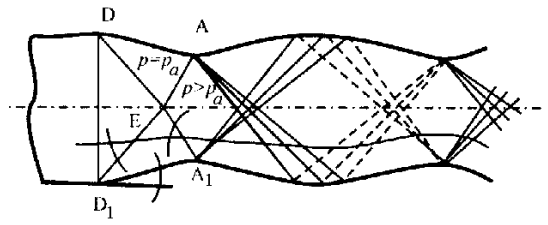
\includegraphics[width = 0.8\textwidth]{Перерасширение.png}
        \caption{Струя идеального газа при перерасширении}
    \end{figure}
    
    \item \textbf{Истечение газа с недорасширением.}  
    В случае, если противодавление меньше, чем давление на срезе, реализуется режим истечения с недорасширением, т.е. как бы из укороченного сопла.
    \begin{figure}[H]\label{fig: underexpansion}
        \centering
        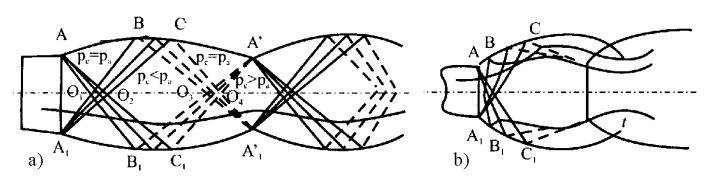
\includegraphics[width = 0.8\textwidth]{Недорасширение.png}
        \caption{a) Схема сверхзвуковой плоской недорасширенной струи идеального газа, b) То же для осесимметричной струи идеального газа}
    \end{figure}
     
\end{enumerate}

\textbf{Экспериментальная установка:}
Схема экспериментальной установки представлена на рис. 1. 
\begin{figure}[H]\label{fig: ustanovka scheme}
    \centering
    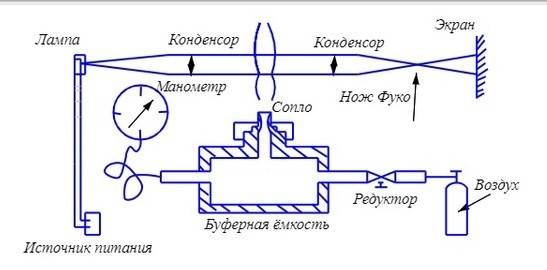
\includegraphics[width = 0.9 \textwidth]{Схема установки.png}
    \caption{Схема экспериментальной установки}
\end{figure}
Воздух из баллона высокого давления через редуктор поступает в ресивер. Ресивер представляет собой толстостенный сосуд объёмом $200 \text { } см^3$, служащий для выравнивания параметров газа в предсопловом объеме. Давление в нём устанавливается и регулируется редуктором. К ресиверу подсоединяются сменные сопла. В работе используется набор осесимметричных конических сопел, позволяющих получать потоки газа с различными числами $M$. Установка оснащена визуализирующей оптической системой, которая может быть построена в полутеневом или шлирном варианте. Она состоит из точечного источника света, набора линз, ножа Фуко и экрана.

\textbf{Методика измерений:}

Давление в ресивире измеряется пружинным манометром. Для измерения распределения полного давления вдоль струи используется насадок полного  давления, соединённый с пружинным манометром.  

\textbf{Обработка данных:} 

\begin{enumerate}
    \item 
    Запишем параметры используемых в работе сопел, значения приведены в таблице ниже.
    \begin{table}[H]\label{tab: nozzles params}
        \centering
        \begin{tabular}{|
            >{\columncolor[HTML]{FFFFFF}}c |
            >{\columncolor[HTML]{FFFFFF}}c |
            >{\columncolor[HTML]{FFFFFF}}c |}
            \hline
            {\color[HTML]{000000} Материал} & {\color[HTML]{000000} $D_{вх.}$, мм} & \cellcolor[HTML]{FFFFFF}{\color[HTML]{000000} $D_{вых.}$, мм} \\ \hline
            {\color[HTML]{000000} Стекло}   & {\color[HTML]{000000} 1,57}          & {\color[HTML]{000000} 1,73}                                   \\ \hline
            {\color[HTML]{000000} Алюминий} & {\color[HTML]{000000} 1,58}          & {\color[HTML]{000000} 2,27}                                   \\ \hline
        \end{tabular}
        \caption{Параметры сопел}
    \end{table}

    \item
    Используя метод последовательных приближений, с помощью первой формулы из \eqref{eq: T P rho ratios} теоретически рассчитаем число Маха для потока воздуха. Для этого Из \eqref{eq: T P rho ratios} выразим $M$, за начальное значение $M_0$ возьмём $M_0 = 1$, тогда 
    \begin{equation}
        \left\{
            \begin{aligned}
                M_0 &= 1, \\
                M_i &= \bigg( \frac{\gamma + 1}{\gamma - 1} \bigg( \frac{A}{A^*} M_{i - 1}\bigg)^{\frac{2(\gamma - 1)}{\gamma + 1}} - \frac{2}{\gamma - 1} \bigg)^{\frac{1}{2}};
            \end{aligned}
    \end{equation}
    Результат вычислений занесём в таблицу.
    \begin{table}[H]\label{tab: teoritical M}
        \centering
        \begin{tabular}{|
            >{\columncolor[HTML]{FFFFFF}}c |
            >{\columncolor[HTML]{FFFFFF}}c |
            >{\columncolor[HTML]{FFFFFF}}c |}
            \hline
            {\color[HTML]{000000} Материал}               & {\color[HTML]{000000} Стекло} & {\color[HTML]{000000} Алюминий}                     \\ \hline
            {\color[HTML]{000000} Число Маха $M$} & {\color[HTML]{000000} 1,55}   & \cellcolor[HTML]{FFFFFF}{\color[HTML]{000000} 2,22} \\ \hline
        \end{tabular}
        \caption{Теоретически рассчитанные числа Маха}
    \end{table}

    \item
    После этого, используя формулы \eqref{eq: T P rho ratios}, с помощью рассчитанных раннее значений числа Маха $M$ получим давление газа в расчётном режиме, а затем сравним с экспериментальными данными.
    \begin{table}[H]\label{tab: teor and exp p_0}
        \centering
        \begin{tabular}{|
        >{\columncolor[HTML]{FFFFFF}}c |
        >{\columncolor[HTML]{FFFFFF}}c |
        >{\columncolor[HTML]{FFFFFF}}c |}
        \hline
        {\color[HTML]{000000} Материал} &
          {\color[HTML]{000000} \begin{tabular}[c]{@{}c@{}}Теоретическое\\ $p$, атм.\end{tabular}} &
          {\color[HTML]{000000} \begin{tabular}[c]{@{}c@{}}Экспериментальное\\ $p$, атм.\end{tabular}} \\ \hline
        {\color[HTML]{000000} Стекло} &
          {\color[HTML]{000000} 3,95} &
          {\color[HTML]{000000} 4,05} \\ \hline
        {\color[HTML]{000000} Алюминий} &
          {\color[HTML]{000000} 11,03} &
          {\color[HTML]{000000} 10,65} \\ \hline
        \end{tabular}
        \caption{Теоретически рассчитанные и экспериментальные значения давления}
    \end{table}

    \item
    Далее измерим давление в ресивире $p_0$ и давление на выходе $p'_0$, после этого, используя метод последовательных приближений, рассчитаем число Маха по полученным значениям давления с помощью формулы
    \begin{equation}
        \left\{
            \begin{aligned}
                M_0 &= M_{геом.}, \\
                M^2_i &= \frac{\gamma - 1}{2 \gamma} + \frac{\gamma + 1}{2 \gamma} \bigg(\frac{p'_0}{p_0}\bigg)^{1 - \gamma} \bigg[ \frac{2}{\gamma + 1} \bigg( \frac{1}{M^2_{i - 1}} + \frac{\gamma - 1}{2}\bigg) \bigg]^{-\gamma}.
            \end{aligned}
    \end{equation}
    где $M_{геом.}$ -- число Маха, рассчитанное первым способом. Сравним полученные двумя способами значения $M$, результаты приведены в таблице ниже:
    \begin{table}[H]\label{tab: M via A and p}
        \centering
        \begin{tabular}{|
            >{\columncolor[HTML]{FFFFFF}}c |
            >{\columncolor[HTML]{FFFFFF}}c |
            >{\columncolor[HTML]{FFFFFF}}c |}
            \hline
            {\color[HTML]{000000} Число Маха} & {\color[HTML]{000000} Через $\frac{A}{A^*}$} & {\color[HTML]{000000} Через $\frac{p'_0}{p_0}$} \\ \hline
            {\color[HTML]{000000} Стекло}     & {\color[HTML]{000000} 1,56}                  & {\color[HTML]{000000} 1,49}                     \\ \hline
            {\color[HTML]{000000} Алюминий}   & {\color[HTML]{000000} 2,22}                  & {\color[HTML]{000000} 2,36}                     \\ \hline
        \end{tabular}
        \caption{Сравнение расчётов по разным формулам}
    \end{table}

    \item
    Последним пунктом пронаблюдаем на практике различные режимы истечения из сопла. Ниже представлены фотографии для каждого случая.
    \begin{figure}[H]\label{fig: exp norm mode}
        \centering
        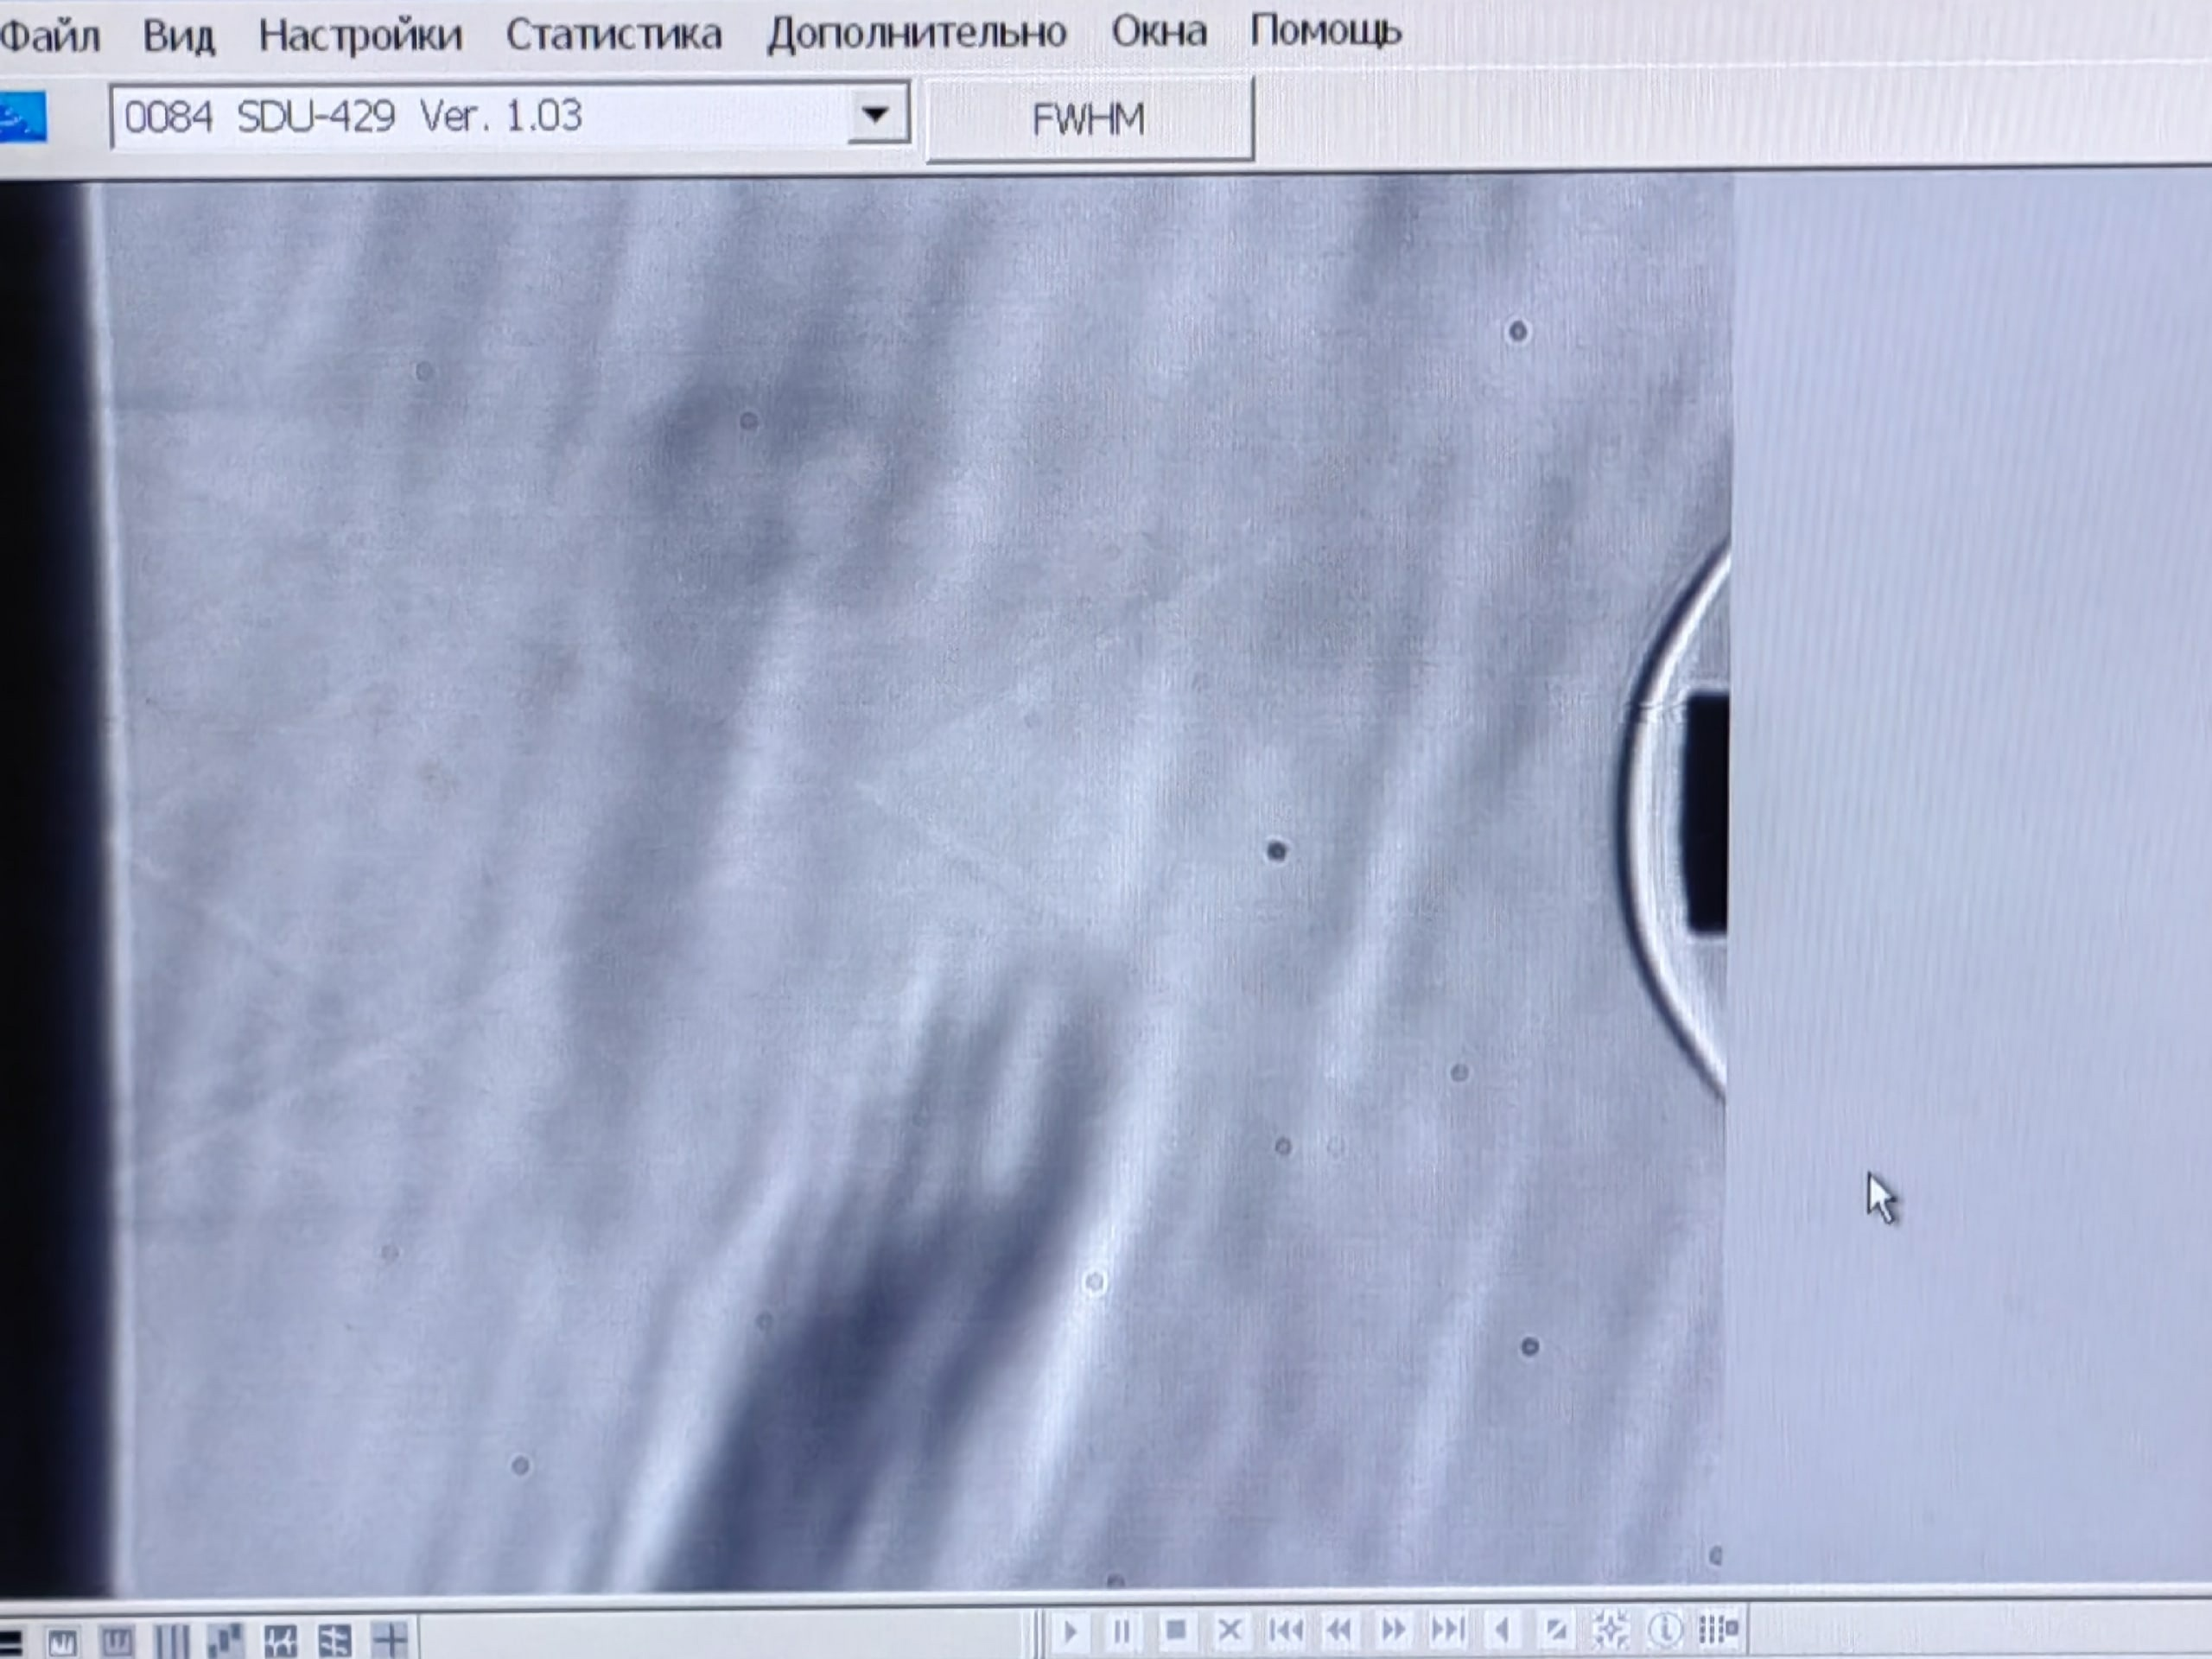
\includegraphics[width = 0.7\textwidth]{Эксп Расчёт.png}
        \caption{Алюминиевое сопло, расчётный режим, $p_0 = 10,65$ атм.}
    \end{figure}
    \begin{figure}[H]\label{fig: exp overexpansion}
        \centering
        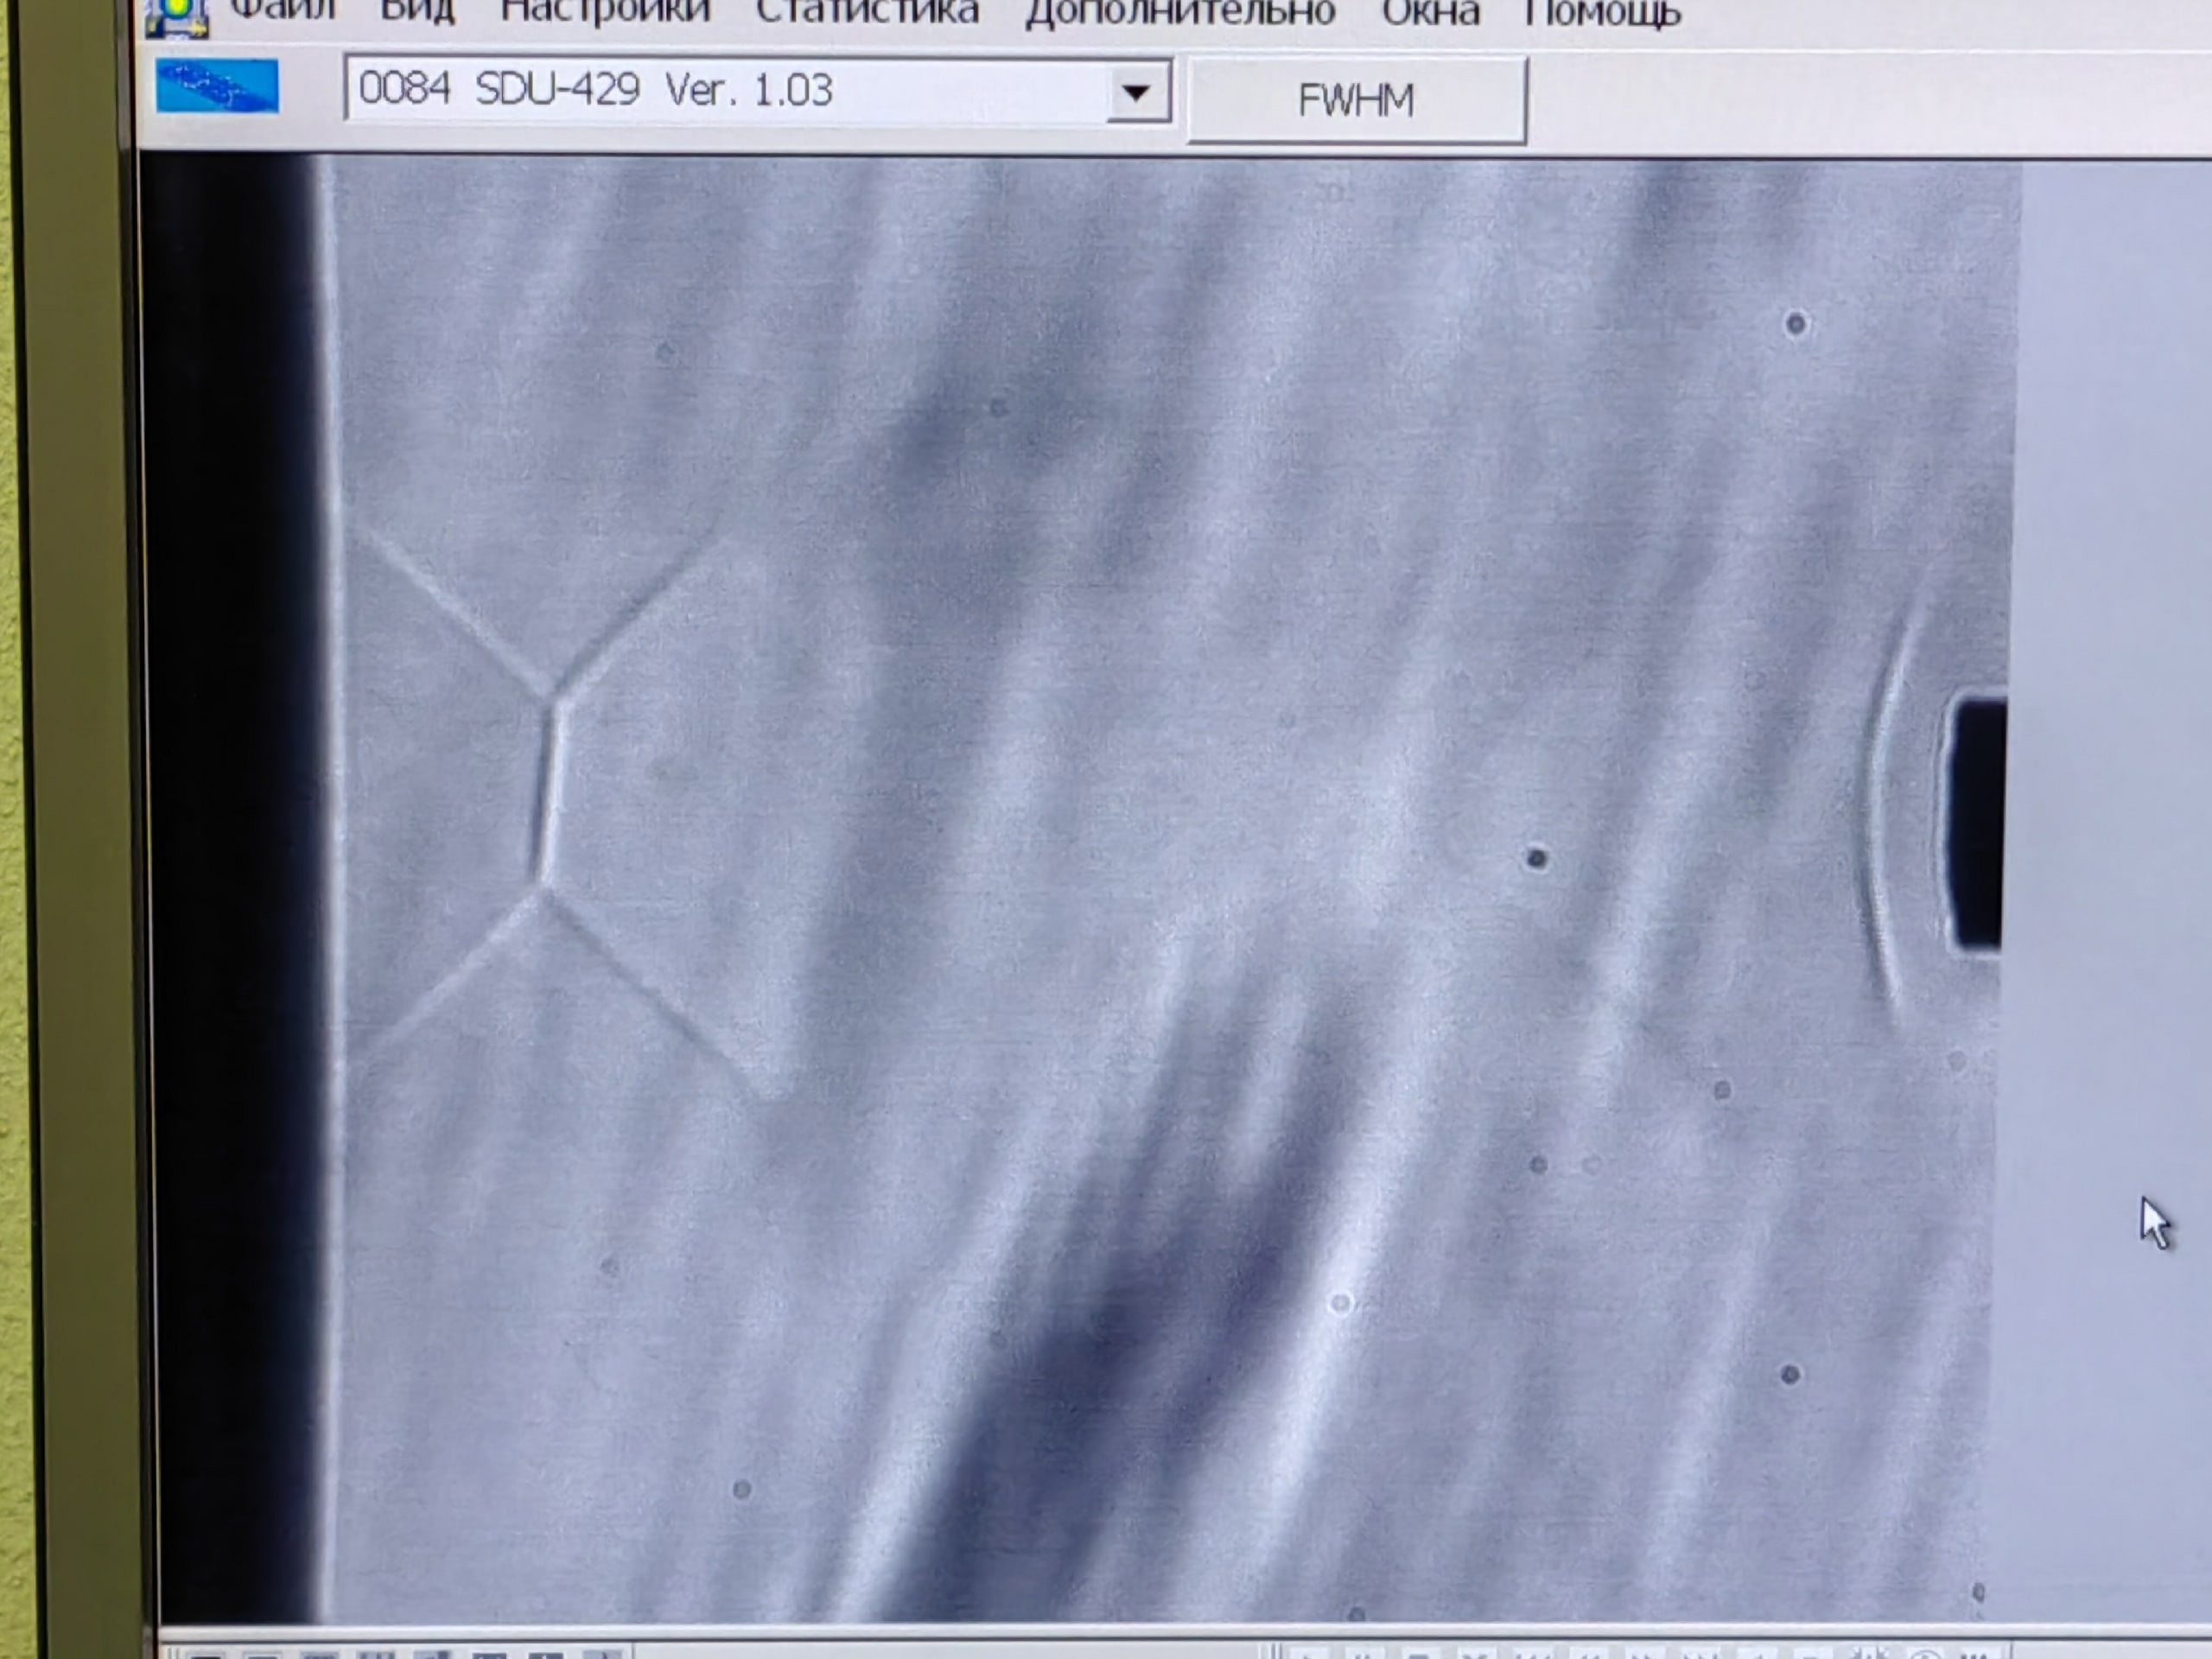
\includegraphics[width = 0.7\textwidth]{Эксп Пере.png}
        \caption{Алюминиевое сопло, режим перерасширения, $p_0 = 5,3$ атм.}
    \end{figure}
    \begin{figure}[H]\label{fig: exp nozzle flow}
        \centering
        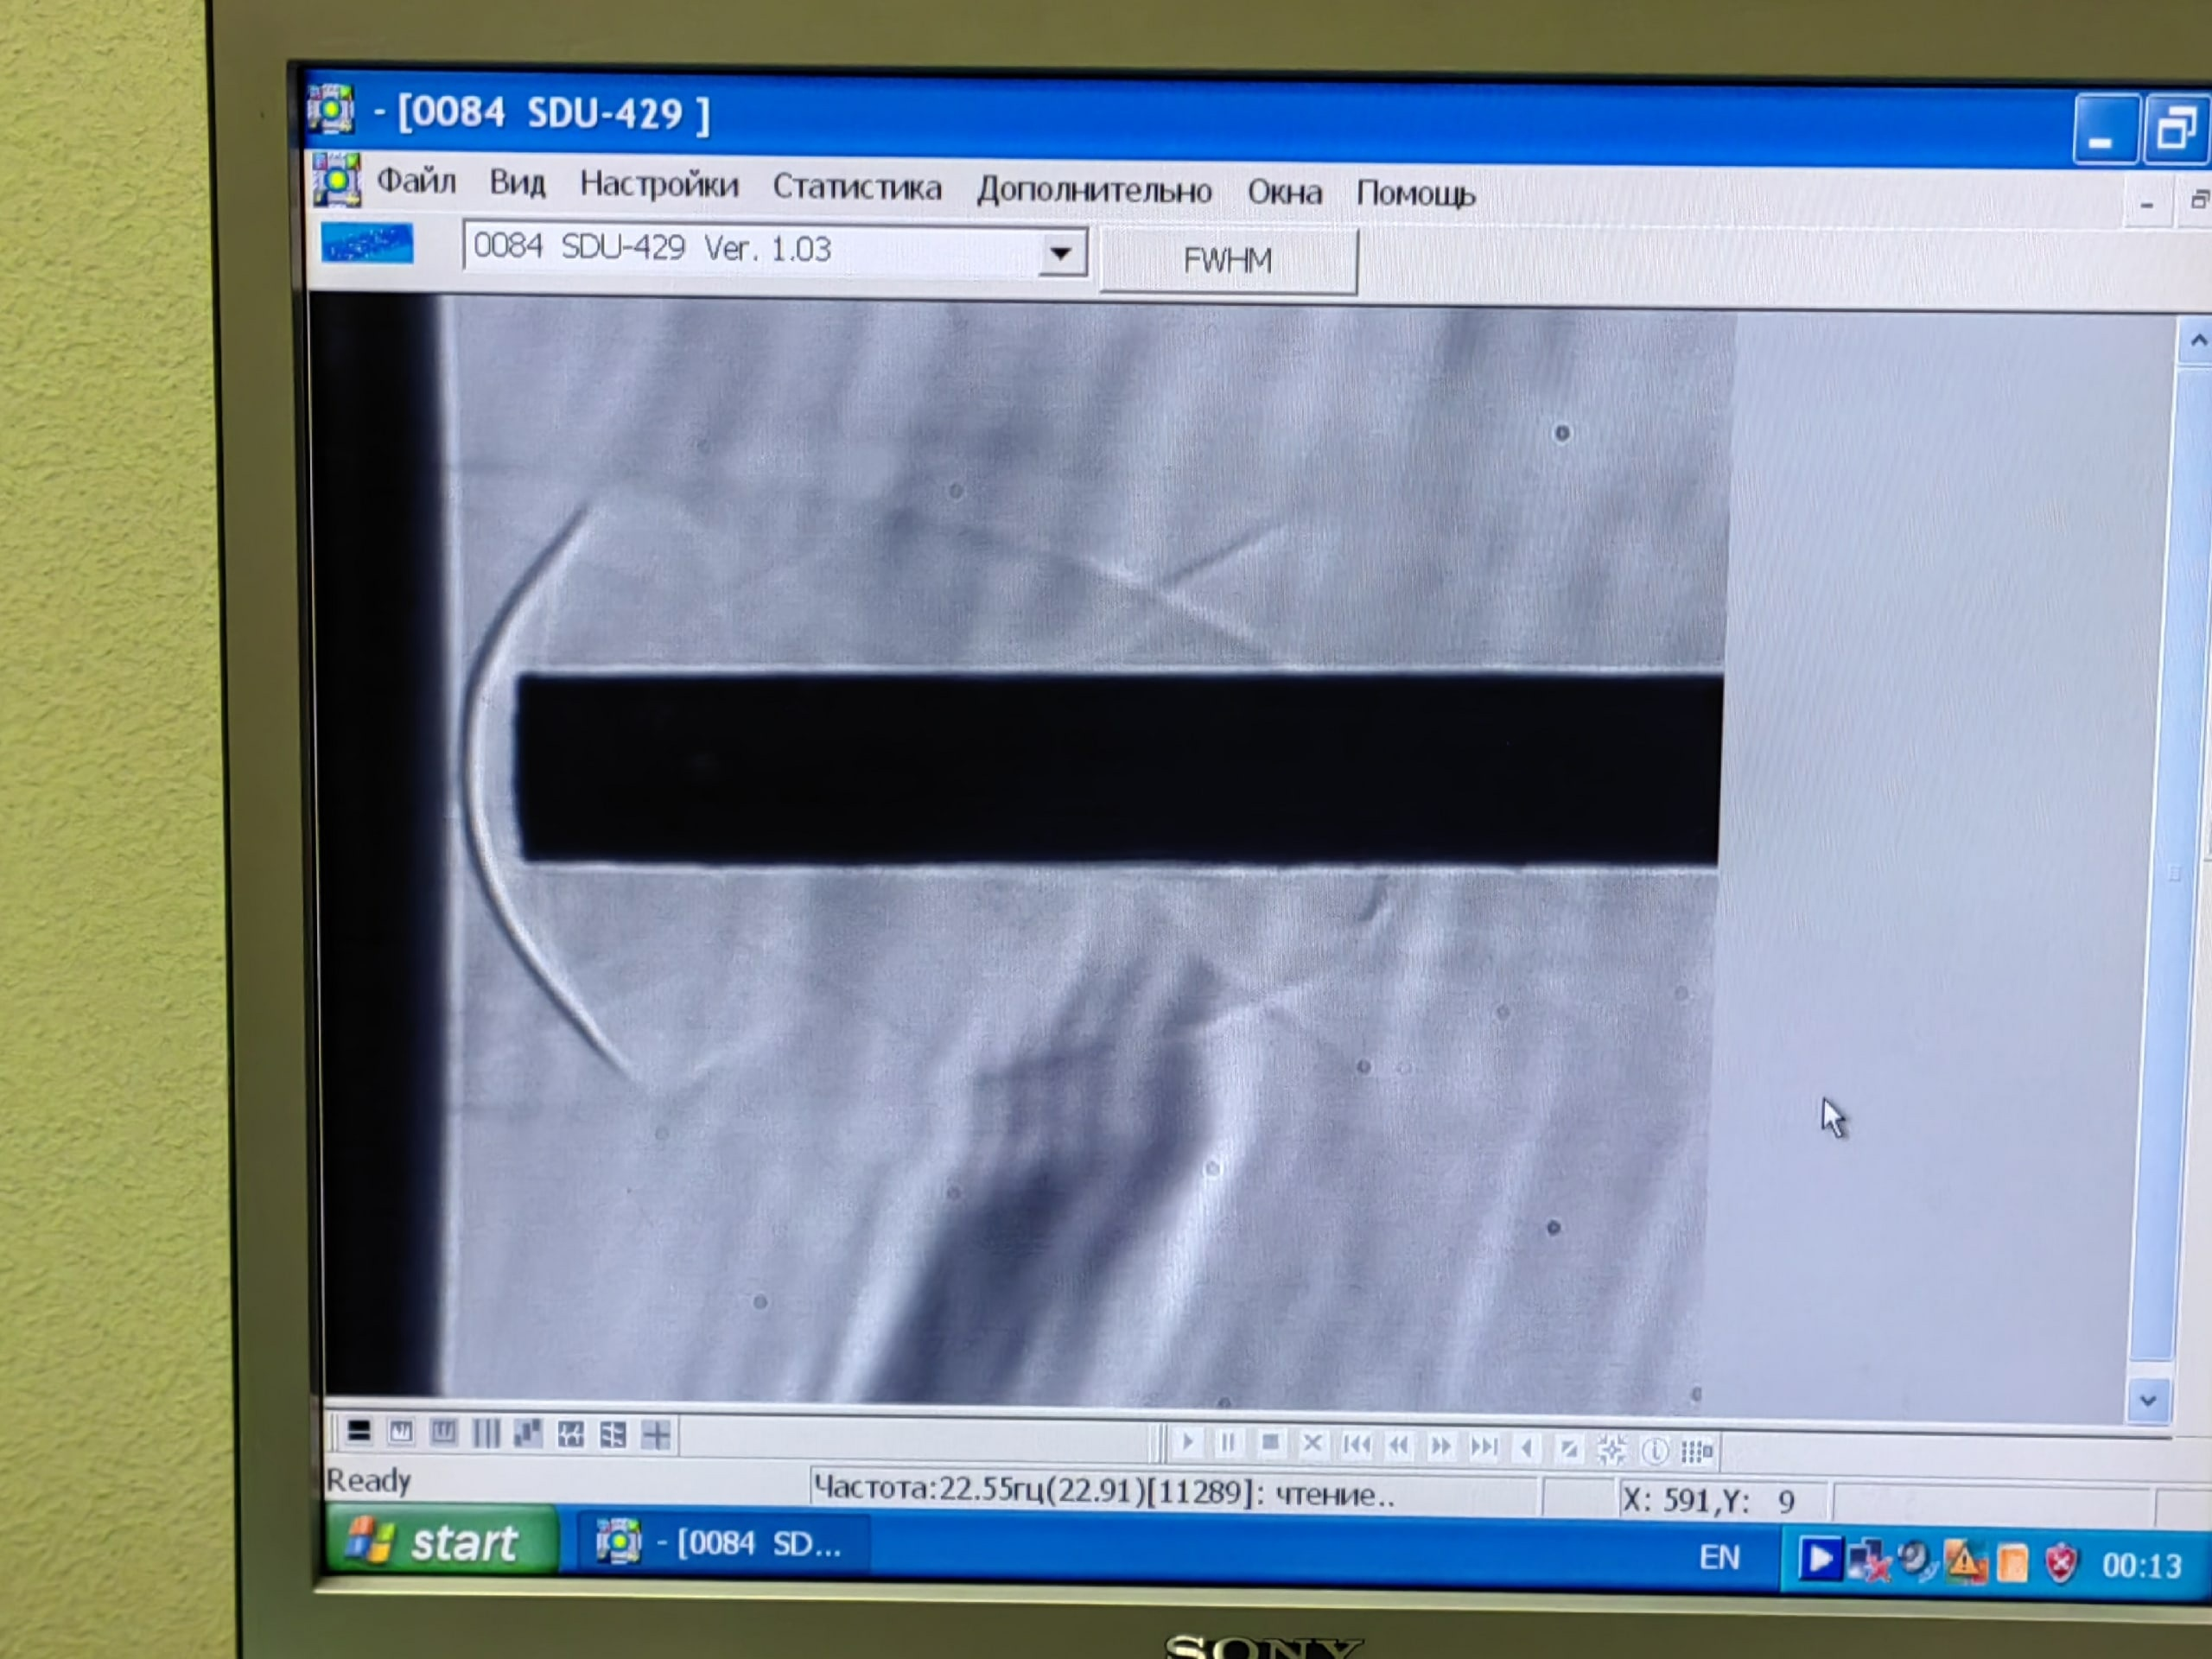
\includegraphics[width = 0.7\textwidth]{Эксп Обтекание насадки.png}
        \caption{Алюминиевое сопло, обтекание насадки, $p_0 = 11$ атм. $p_0' = 6,1$ атм.}
    \end{figure}
    
\end{enumerate}

\textbf{Вывод:} 
В данной работе был изучен процесс истечения газа из сопла Лаваля в приближении одномерной теории адиабатического изоэнтропического истечения. В работе использовались два различных сопла (стеклянное и алюминиевое), для каждого из них было вычислено значение числа Маха $M$ двумя способами (с помощью геометрии сопел и с помощью разности давлений на входе и выходе из сопла), также, на опыте были рассмотрены и проанализированы три различных режима истечения из сопла (с недорасширением, расчётный, с перерасширением).

\end{document}
